\chapter{Zona de estudio.}
La zona de estudio se encuentra localizada en las afueras del per\'imetro urbano del municipio de Ciudad Bol\'ivar en el Departamento de Antioquia. 
Las laderas noroxidental y suroriental de la quebrada la linda abarcan un \'area de xx metros cuadrados con pendientes que oscilan entre el 20\% y 30\%
 La Quebrada La Linda no posee afluente alguno, sus aguas se desembocan en La Quebrada La Raya.
Las pendientes m\'as pronunciadas de la cuenca hidrogr\'afica de la Qda. La Linda se encuentran aguas arribas en, hacia las cercan\'ias del Batolito Farallones, tal como se puede apreciar en la figura \ref{fig:slopes}

\begin{figure}[H]
\centering
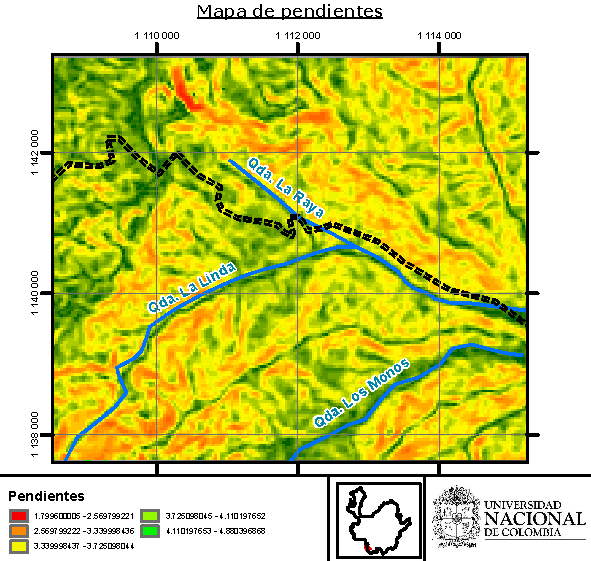
\includegraphics[scale=1]{img/pendientes.pdf}
\caption{Mapa de pendientes de la cuenca hidrogr\'afica de la Qda. La Linda y sus zonas circundantes. Elaboraci\'on propia}

Para el tratamiento de esta cuenca hidrogr\'afica no seha realizado separaci\'on de UMI (Unidad Morfodinamica independiente) por los siguientes motivos
\label{fig:slopes}
\end{figure}
La principal v\'ia de acceso es la carretera que desde el municipio de Ciudad B\'olivar conduce a El Carmen de Bol\'ivar.